\chapter{Experimental results preview}

Since its introduction, the theory of perturbative Quantum Chromodynamics (pQCD) has made huge strides and its calculations for the strong coupling constant
are improving by the inclusion of higher order terms in the power series. However, the non-perturbative regime is still poorly understood as numerical
calculations on a lattice fail to describe dynamical factors such as transport coefficients and cross sections, as opposed to outlining light nuclei
and hadron spectra. Therefore, to further the understanding of QCD under extreme temperatures and baryon densities, experiments involving high energy
particle collisions pave the way for development of new theoretical tools to describe the phenomena in a new light.

\section{Ion collider experiments}
The experimental endeavours in the search for a deconfined state of matter began as early as 1986 with fixed target experiments at the Alternating Gradient
Synchrotron (AGS) at Brookhaven National Laboratory (BNL) and the Super Proton Synchrotron (SPS) at CERN. Beginning with light atomic nuclei like $^{16}$O,
$^{28}$Si and $^{32}$S, the focus of the experiments shifted towards heavier nuclei collisions involving $^{197}$Au and $^{208}$Pb in the 1990's. The
AGS demonstrated centre-of-mass energy per colliding nucleon pair of $\sqrt{s_{\textnormal{\sc nn}}}$ = 4.6 GeV while the SPS achieved
$\sqrt{s_{\textnormal{\sc nn}}}$ = 17.2 GeV in Pb-Pb collisions\cite{MunzingerStachel:2007} and $\sqrt{s_{\textnormal{\sc nn}}}$ = 19 GeV in S-S
collisions\cite{Evans:1999}. The results from SPS experiment at CERN gathered enough evidence to conclude a new state of matter had been
created\cite{SPSqgp:2000, HeinzLHC:2000}.

Concurrently, a new accelerator with much higher collision energies went into operation at BNL. The Relativistic Heavy-Ion Collider (RHIC) made it possible
to reach centre-of-mass energies $\sqrt{s_{\textnormal{\sc nn}}}$ = 200 GeV by colliding heavy nuclei such as gold and servicing four experiments called
BRAHMS, PHENIX, PHOBOS and STAR. The higher collision energies reached at RHIC meant a significantly larger and hotter fireball was possible. From the
experiments at RHIC, it was concluded that QGP is not a gas-like plasma but is a strongly interacting near-perfect fluid\cite{Adams:2005}.

The initiation of LHC set a new world-record for heavy ion collisions at $\sqrt{s_{\textnormal{\sc nn}}}$ = 2.76 TeV per nucleon for Pb-Pb during its first
run (2010--2013), and $\sqrt{s_{\textnormal{\sc nn}}}$ = 5.02 TeV per nucleon for Pb-Pb during Run 2 (2015--2018). This allowed a deeper study of the QGP
phase and its properties owing to more extreme conditions and a detailed characterisation of hadronisation and particle generation as the fireball cools down.
An in-depth overview of the LHC and the ALICE experiment focusing on QGP study is provided in Chapter \ref{sec:LHC}.

\section{Experimental Observables}

Since the QGP cannot be observed directly at present, external observables are used to gauge information about the particles produced in the
collisions. These observables, called probes, can be categorised into two types: soft and hard probes. Soft probes characterise the macroscopic and
collective behaviour of particles and the collision as a whole, while hard probes allow energy loss studies within the QGP and are sensitive to strong
interaction at the partonic level.

\subsection{Collective flow and correlations}
Anisotropies observed in the final momentum distribution of particles created in nuclear collisions suggest the presence of collective behaviour in the
formed system. Initially proposed as a signature of QGP's collective behaviour, in-plane elliptic flow was experimentally observed at
AGS\cite{FlowAGS:1994} and SPS\cite{FlowSPS:2003}. A strong elliptic flow measured at RHIC clarified QGP's resemblance to a strongly interacting
liquid\cite{Adams:2005}.

The initial overlap region of colliding nuclei plays a major role in anisotropies in momentum distribution as different pressure gradients form along
different axes. These anisotropies can be quantified using the Fourier coefficients of the azimuthal particle distributions:

\begin{equation}
    v_{n} = \langle cos[n(\phi - \Psi_{n})]\rangle
    \label{eq:fourier}
\end{equation}

where $n$ is the flow harmonic order, $\phi$ is the azimuthal angle of the particle, and $\Psi_{n}$ is the angle of the initial state spatial plane of
symmetry\cite{Voloshin:1996, Fourier:2011}. The first, second and third harmonics indicate directed, elliptic and triangular flow respectively.
The elliptic flow coefficient $v_{2}$ signifies the difference between pressure gradients, although higher order coefficients also help in decrypting
the initial state geometry and the fireball's evolution.

Flow measurements allow constraints to be put on equation of state and enable kinematic viscosity measurements, $\eta/s$, defined as ratio of shear
viscosity to entropy density. $\eta/s$ value for a perfect fluid has a lower limit of $\frac{1}{4\pi}$\cite{Viscosity:2005}(natural units). Experimental
values from RHIC and ALICE, LHC are consistent with $\eta/s$ = 0.12 and $\eta/s$ = 0.2 respectively\cite{Gale:2013} (Fig. \ref{fig:viscosity}). The low $\eta/s$ values
point towards QGP's status as a near-perfect fluid and differences between results from RHIC and ALICE allow determination of temperature dependence of
kinematic viscosity.
\begin{figure}[H]
    \centering
    \begin{subfigure}{.5\textwidth}
        \centering
        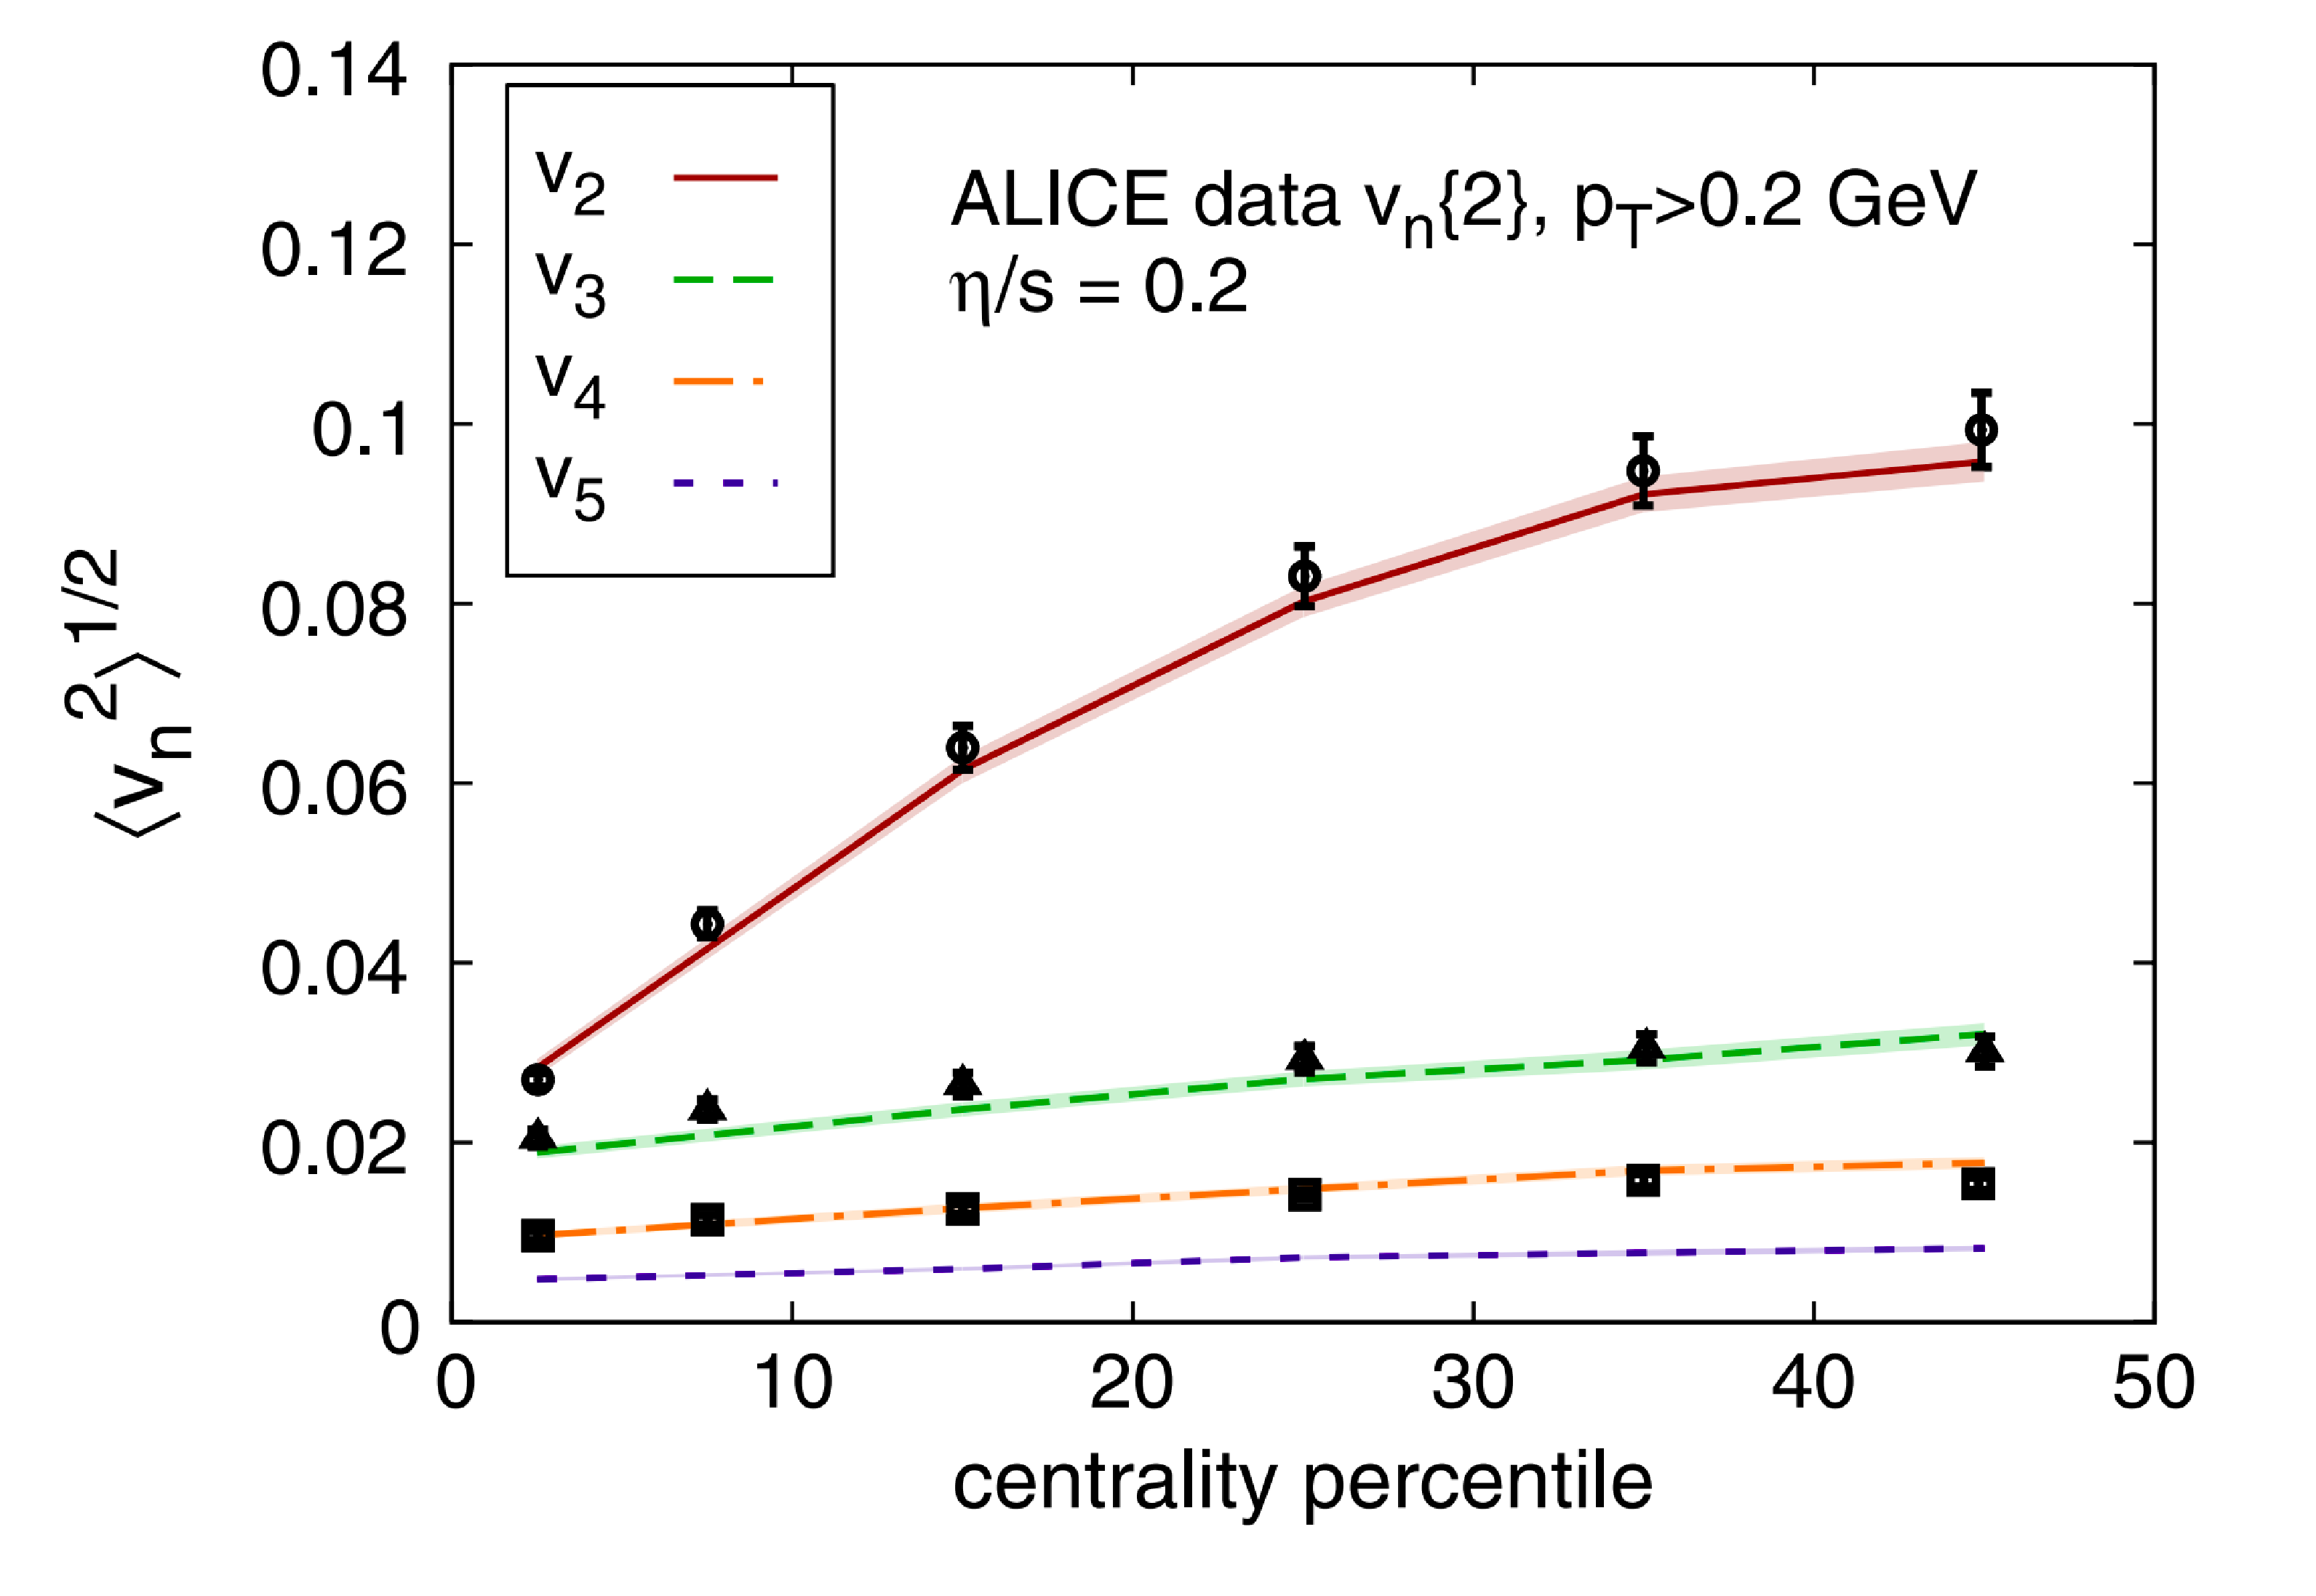
\includegraphics[width=\linewidth]{images/aliceViscosity.pdf}
    \end{subfigure}%
    \begin{subfigure}{.5\textwidth}
        \centering
        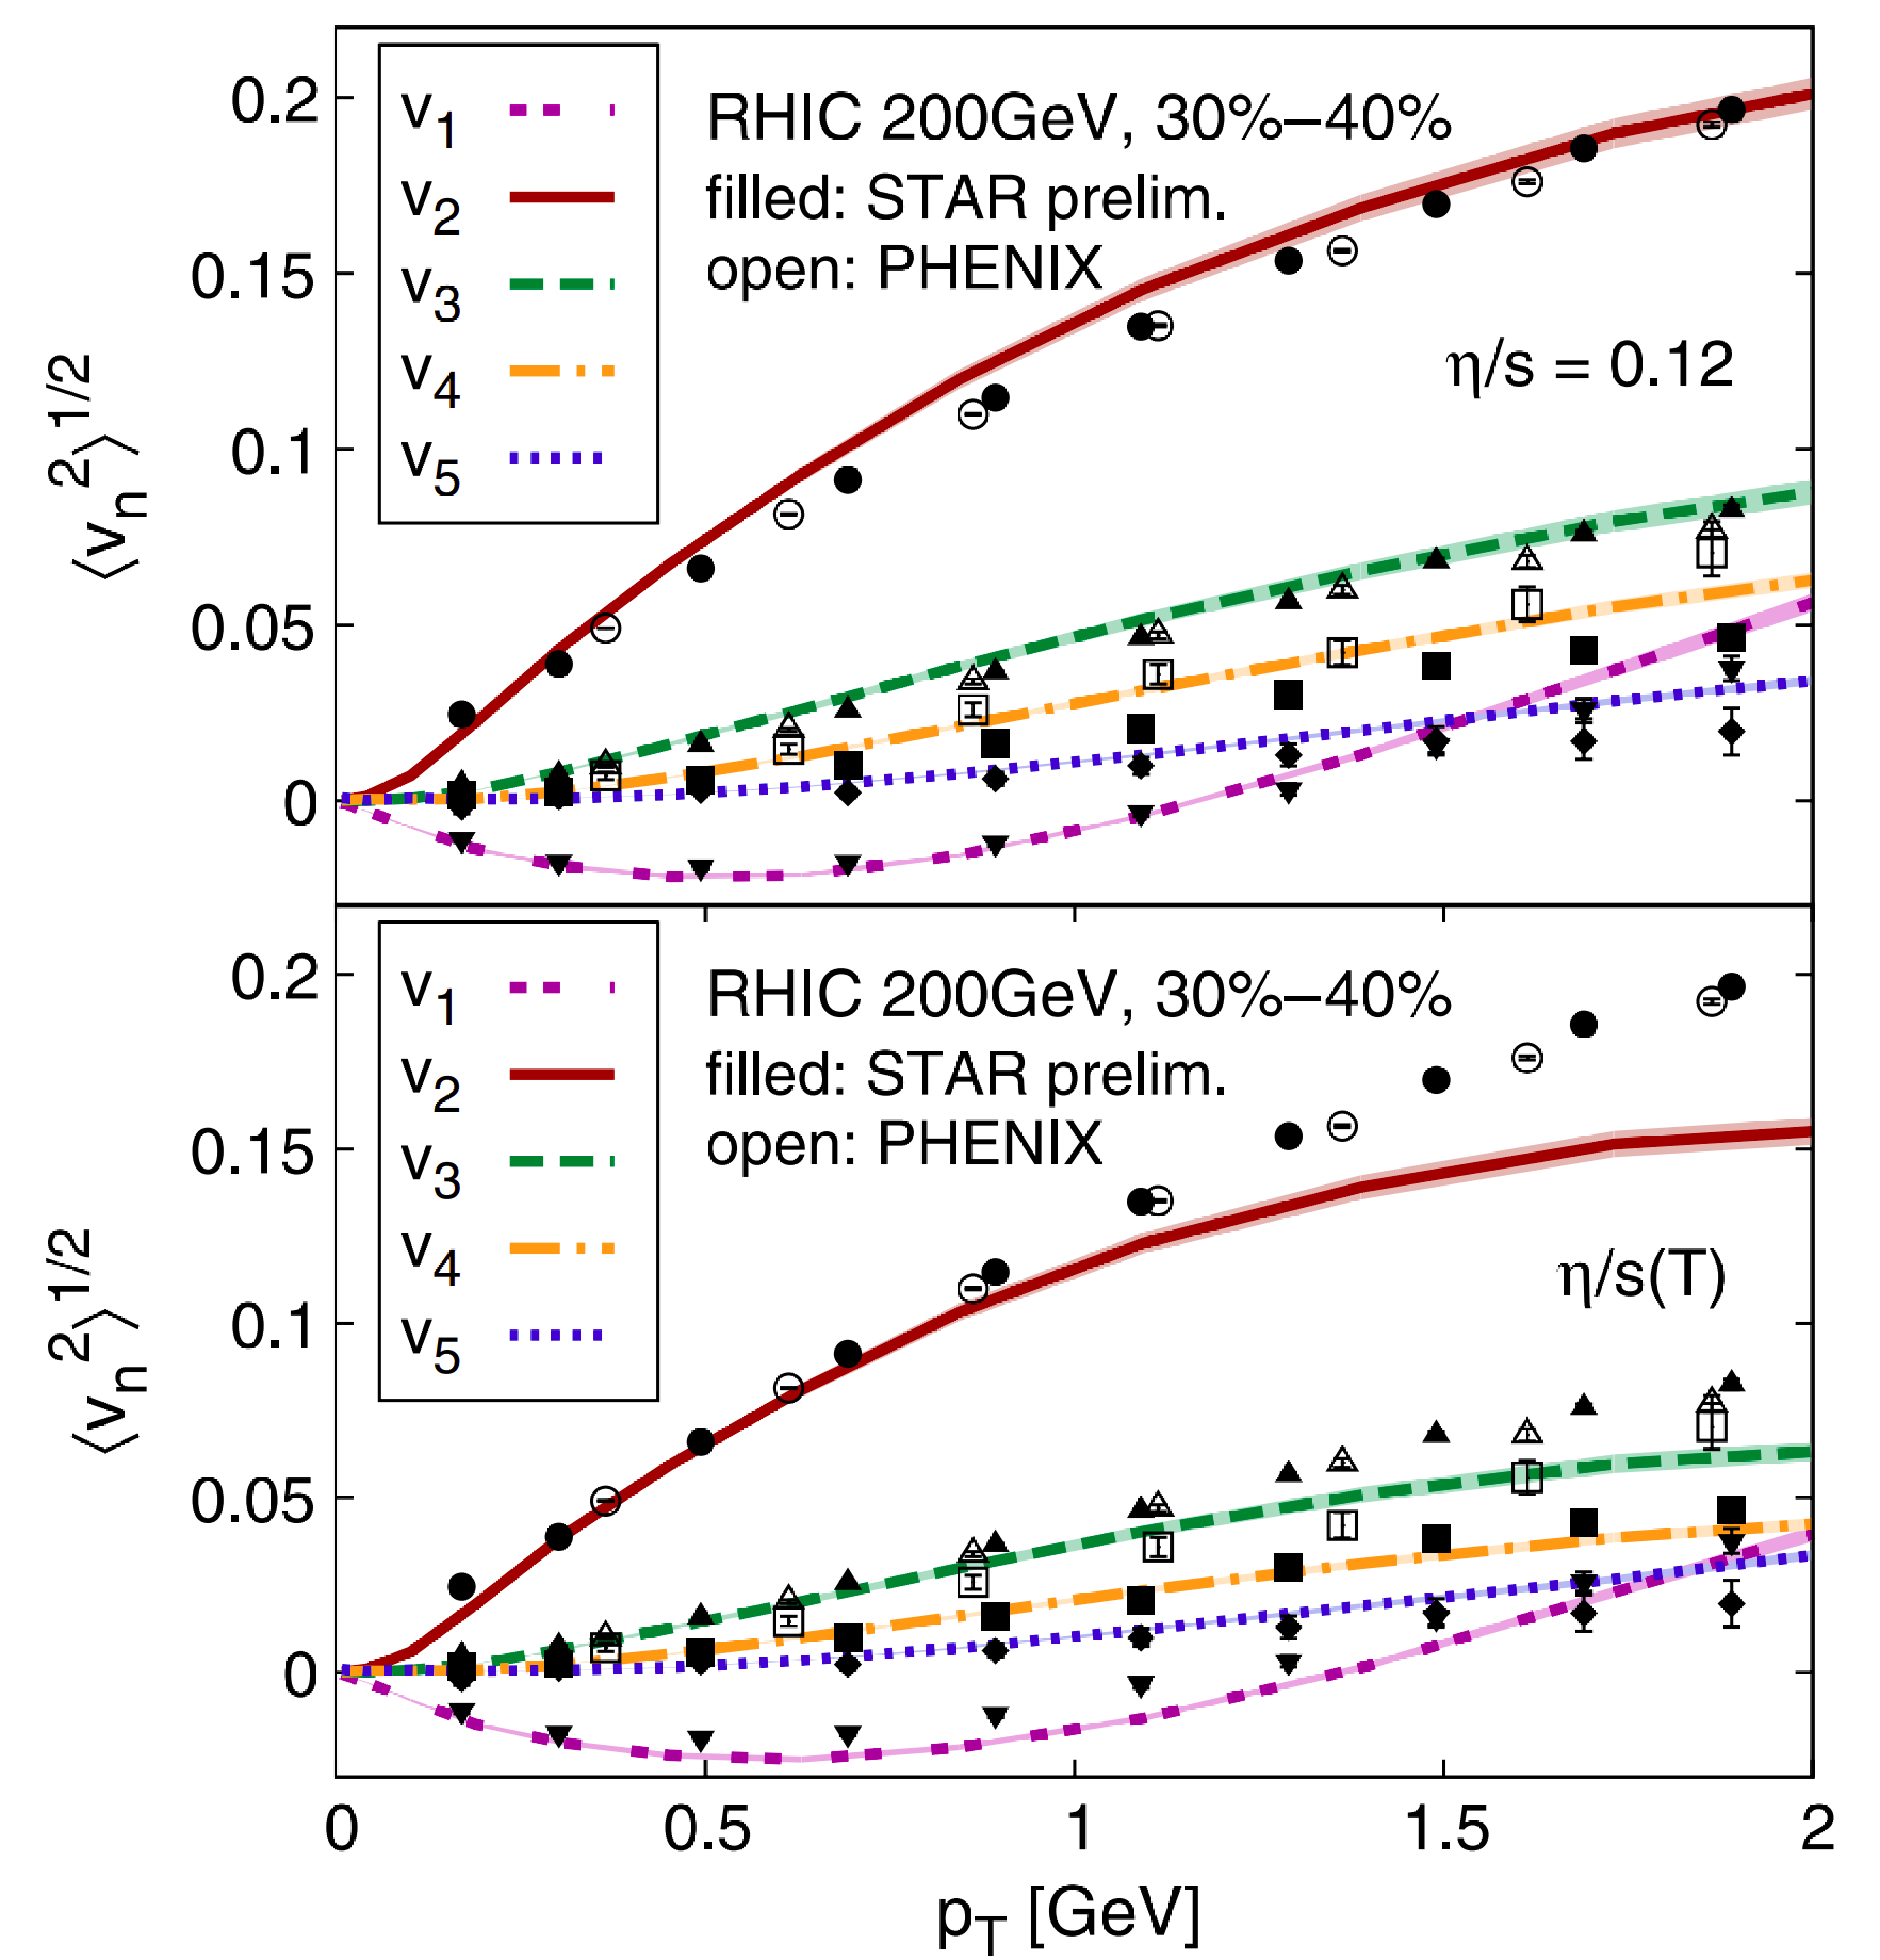
\includegraphics[width=\linewidth]{images/rhicViscosity.pdf}
    \end{subfigure}
    \caption{RMS values of anisotropic flow coefficients $\langle v_{n}^{2}\rangle^{1/2}$. Left plot from ALICE Collaboration depicts $\langle v_{n}^{2}\rangle^{1/2}$
        computed as a function of centrality\protect \footnotemark \ and compared to experimental data based on $v_{n}\{2\}, n\in 2,3,4$. Plot on the right from the PHENIX and 
        STAR collaboration shows a comparison
        of $v_{n}(p_{\textnormal{\sc t}})$ at RHIC using a constant $\eta/s$ = 0.12 (top) and a temperature
        dependent $\eta/s$(T) (bottom)\cite{Gale:2013}.}
    \label{fig:viscosity}
\end{figure}
\footnotetext{centrality of a collision is expressed as a percentage of total nuclear interaction cross section}

When deviating from central collisions, the overlap region of the colliding nuclei becomes less circular and more almond shaped. This increase in spatial
anisotropy results in an increased elliptic flow, as seen in LHC's measurements in Fig. \ref{fig:viscosity} on the left. Higher LHC energies enable elliptic flow to be examined
in detail, in conjunction with higher flow harmonics which can shed a light on initial collision conditions and viscosity of the medium.

\subsection{Jet quenching}

In a hard scattering process (high momentum transfer), the fragmentation of a highly energetic parton results in a collimated spray of hadrons called a
jet. The involved partons, after scattering and hadronization, retain a significant amount of the initial beam momentum and are thus emitted in a narrow
"jet cone". A jet cone can be experimentally identified as a stream of high energy particles moving in approximately the same direction. The hadron in a
jet carrying the highest value of energy is called the leading particle of the jet.

Jet quenching refers to the collisional or radiative energy loss of high energy partons when passing through a hot and dense medium, such as the QGP. The
resulting lower than expected momenta of hadrons produced through hard scattering events leading to a suppression of jets in heavy ion collisions has been
proposed as a key signature of QGP formation\cite{Bjorken:1982}. Various factors determine the energy loss of the jet including the type of parton (quark
or gluon), its energy and mass, the mechanism of energy loss (collisional or radiative), and also medium-induced factors such as the path length and properties
of the medium (size, temperature, coupling). Collisional energy loss occurs due to elastic parton-parton scattering involving a high energy parton, while
radiative energy loss is due to medium-induced gluon radiation.

Experimentally, parton energy loss can be observed through suppression of jet and leading particle spectra by comparing nuclei collision results (QCD medium)
with proton collision results (QCD vacuum). This ratio is stated as the nuclear modification factor, $R_{\textnormal{\sc aa}}\colon$

\begin{equation}
    R_{\textnormal{\sc aa}} \sim \frac{\textnormal {QCD Medium}}{\textnormal{QCD Vacuum}}\sim \frac{\textnormal{AA}}{\textnormal{pp}}
    \label{eq:RAA1}
\end{equation}

\begin{equation}
    R_{\textnormal{\sc aa}} (p_{\textnormal{\sc t}}) = \frac{\textnormal{d}N_{\textnormal{\sc aa}}/\textnormal{d}p_{\textnormal{\sc t}}}{\langle N_{\textnormal{coll}}\rangle\textnormal{d}N_{\textnormal {pp}}/\textnormal{d}p_{\textnormal{\sc t}}}
    \label{eq:RAA2}
\end{equation}

The nuclear modification factor provides the ratio of charged particle yield ($N$) in heavy-ion collisions vs. pp collisions, as a function of
transverse momentum $(p_{\textnormal{\sc t}})$. $\langle N_{\textnormal{coll}}\rangle$ is a theoretical parameter signifying the average number of binary
nucleon-nucleon collisions based on collision centrality.

$R_{\textnormal{\sc aa}}$ equals unity if there are no initial or final state nuclear effects. For jet quenching, the value of $R_{\textnormal{\sc aa}} < 1$
drops below unity. As shown in Fig. \ref{fig:raa}\cite{Raa:2010}, ALICE measurements from Pb-Pb collisions at $\sqrt{s_{\textnormal{\sc nn}}}$ = 2.76 TeV exhibit a significant amount of jet quenching
for the central collisions as compared to the peripheral ones, with $R_{\textnormal{PbPb}} \approx 0.2$ at $p_{\textnormal{\sc t}}
    \approx 7$ GeV/$c$. The results are in agreement with STAR and PHENIX experiments, indicating the formation of QGP.

\begin{figure}[H]
    \centering
    \begin{subfigure}{.5\textwidth}
        \centering
        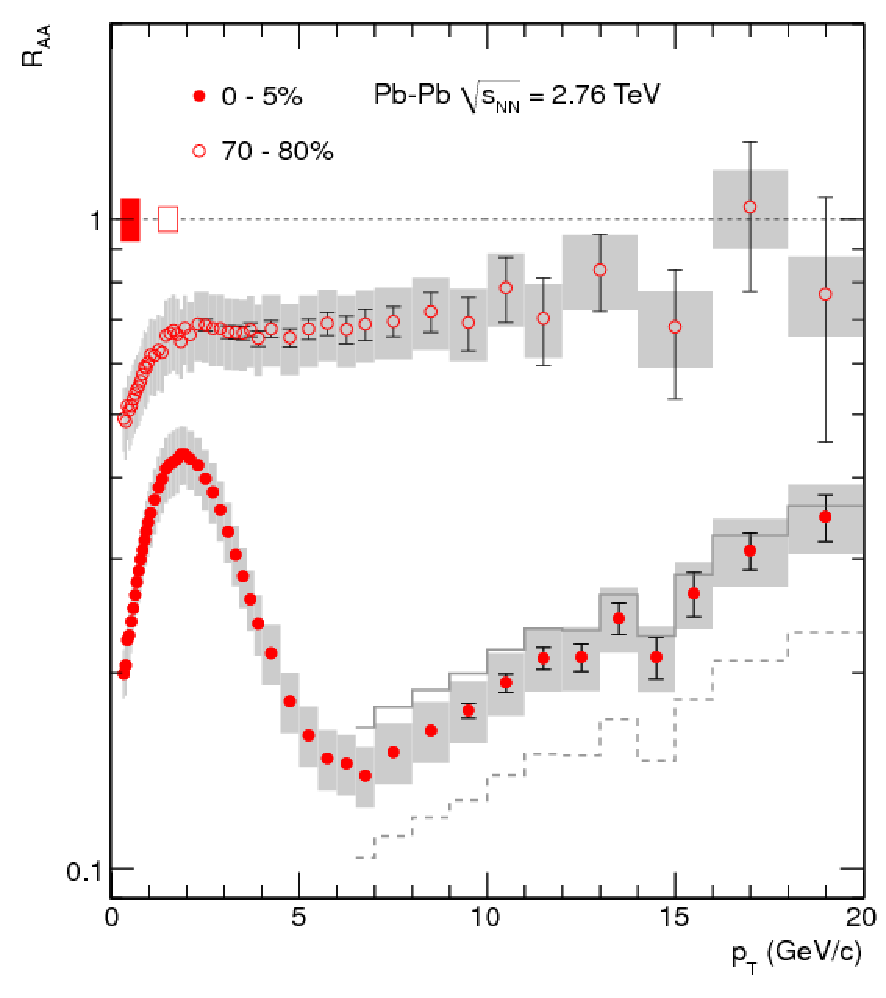
\includegraphics[width=0.85\linewidth]{images/Raa.pdf}
    \end{subfigure}%
    \begin{subfigure}{.5\textwidth}
        \centering
        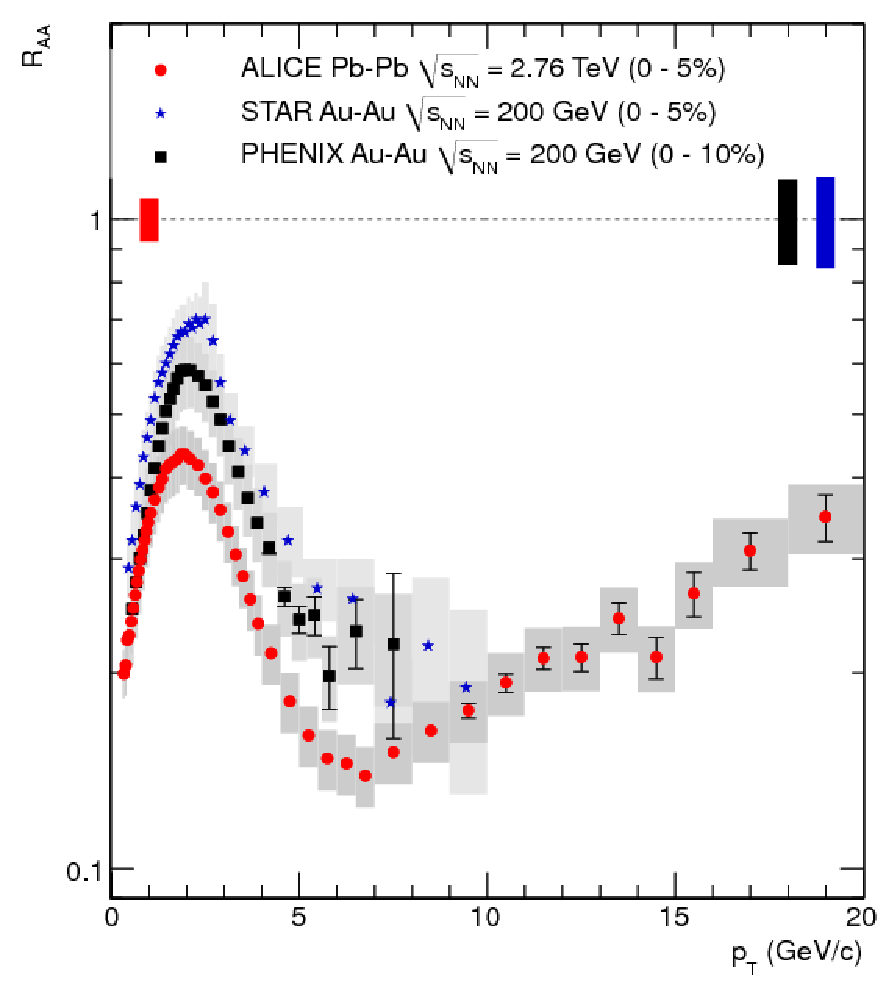
\includegraphics[width=0.85\linewidth]{images/CompRaa.pdf}
    \end{subfigure}
    \caption{Nuclear modification factor ($R_{\textnormal{\sc aa}}$) plots for central $(0-5\%)$ and peripheral $(70-80\%)$ Pb-Pb collisions at
        $\sqrt{s_{\textnormal{\sc nn}}} = 2.76$ TeV in ALICE (left). The central collision results are compared to Au-Au at $\sqrt{s_{\textnormal{\sc nn}}} = 200$
        GeV measurements from STAR and PHENIX (right)\cite{Raa:2010}.}
    \label{fig:raa}
\end{figure}

$R_{\textnormal{\sc aa}}$ measurements in p-Pb collisions at ALICE\cite{sami:2016} yield a value of unity consistent within systematic uncertainties across the
$p_{\textnormal{\sc t}}$ range, essentially disregarding any jet quenching and, therefore, QGP formation. Fig. \ref{fig:raappb} illustrates $R_{\textnormal{pPb}}$
measurements from ALICE at $\sqrt{s_{\textnormal{\sc nn}}} = 5.02$ TeV in blue beside $R_{\textnormal{PbPb}}$ results for central (red) and peripheral
collisions (green). It remains to be seen if Run 2 p-Pb collisions at higher energies $\sqrt{s_{\textnormal{\sc nn}}} = 8.16$ TeV conforms to these results.

\begin{figure}[H]
    \centering
    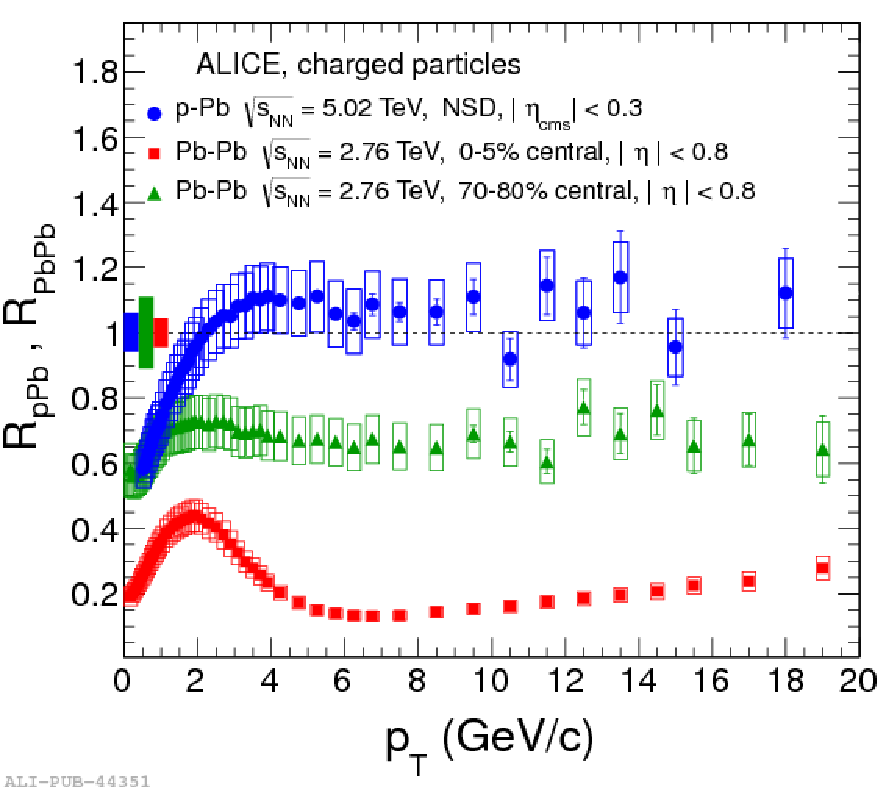
\includegraphics[width=0.7\linewidth]{images/Raappb.pdf}
    \\
    \caption{$R_{\textnormal{\sc aa}}$ for p-Pb collisions at $\sqrt{s_{\textnormal{\sc nn}}} = 5.02$ TeV (blue) compared with $\sqrt{s_{\textnormal{\sc nn}}}
            = 2.76$ TeV Pb-Pb central (red) and peripheral (green) collisions\cite{sami:2016}.}
    \label{fig:raappb}
\end{figure}

\subsection{Strangeness Enhancement}
One of the earliest suggested signatures for the formation of QGP was an increased yield of strange quark production in QGP as compared to a hadronic gas
phase in similar thermodynamic conditions.\cite{Muller:1982}. In the event of a deconfined phase of quarks and gluons (QGP), strange quark pairs production
($s\bar{s}$) can
be abundantly realised through gluon-gluon collisions ($gg \rightarrow s\bar{s}$) or light quark-antiquark annihilation ($q\bar{q} \rightarrow s\bar{s}$).
Strange quark pair production can even reach levels of saturation, i.e. the rate of $s\bar{s}$ annihilation matches its rate of formation, provided the
lifetime of the plasma is long enough. However, strange hadron production is much less abundant owing to a far higher energy threshold as compared to
strange quark pair production as hadron gases follow the hadronic degrees of freedom, rather than partonic. Therefore, strange hadron production
is touted as a signature for QGP formation, and can be observed by comparing strange hadron yields over pion yields in heavy-ion collisions to smaller
systems where QGP formation is not presumed, such as proton-proton and proton-ion collisions.

Earliest experimental indications for strangeness enhancement were observed for enhanced strange Kaon production at AGS, BNL\cite{AGS_Strangeness:1999}
and SPS, CERN\cite{Str_SPS1:1999,Str_SPS2:1999}. Strangeness enhancement was also measured for $\Lambda$\cite{Str_lambda:1989}, $\Xi$\cite{Str_Xi:1991},
and $\Omega\cite{Str_omega}$ particles at SPS. The strangeness content of a particle was predicted to be directly proportional to its expected enhancement.
Thus, the $\Omega$ baryon is expected to be the most enhanced due to this phenomenon, which was later experimentally confirmed\cite{Str_om2:1999}. This
was further verified at different energies and in different ion collision experiments, including LHC\cite{Str_LHC:2013}. Hyperon-to-pion ratios as a
function of average number of participating nucleons in a collision, $\langle N_{\textnormal{part}} \rangle$, measured at ALICE are depicted in Fig.
\ref{fig:hyp}.

\begin{figure}[H]
    \centering
    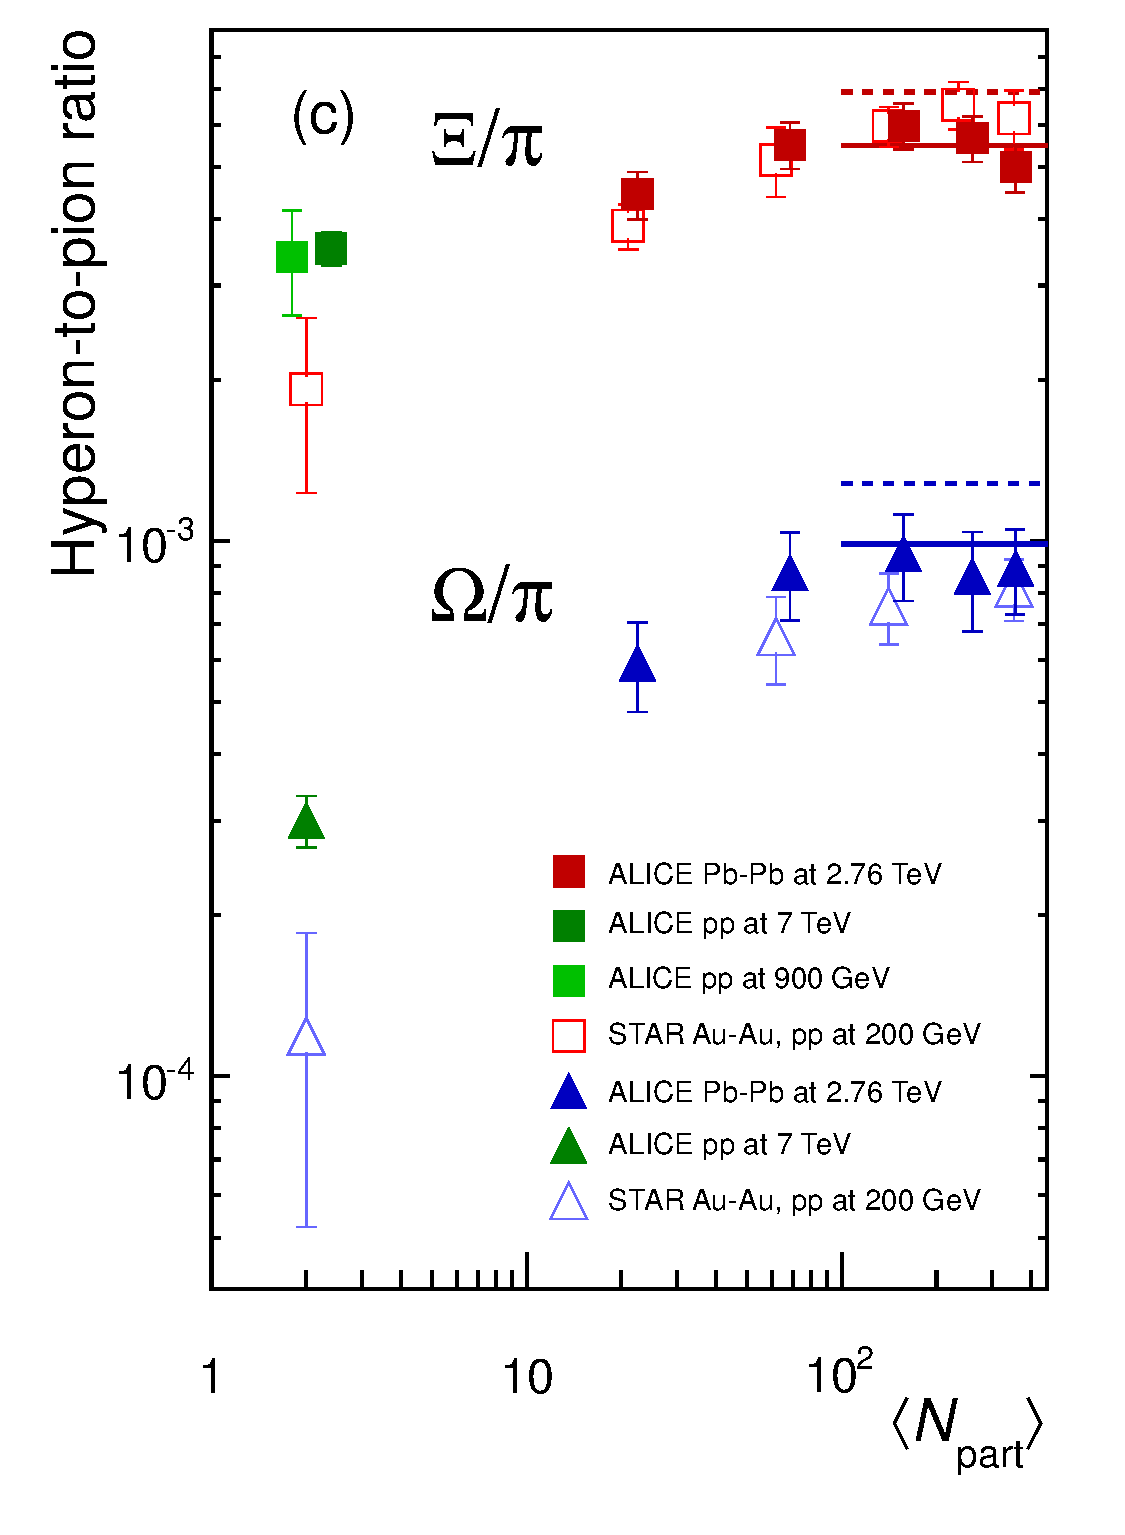
\includegraphics[width=0.5\linewidth]{images/hypToPion.pdf}
    \\
    \caption{Hyperon-to-pion ratios in Pb-Pb and p-p collisions as a function of $\langle N_{\textnormal{part}} \rangle$, ALICE. Results from STAR for
        comparison. Lines indicate thermal model predictions.\cite{Str_LHC:2013}}
    \label{fig:hyp}
\end{figure}

From the figure, the enhancement in Pb-Pb results is apparent as compared to p-p collisions. Results from STAR collaboration represented by open symbols
are plotted for comparison. The enhancement is comparatively weaker at LHC due to higher energy of p-p measurement taken as a reference.

Smaller systems such as proton-proton and proton-ion require a more detailed look, and instead of
$\langle N_{\textnormal{part}} \rangle$, the strange hadron yields were measured as a function of mean charged-particle multiplicity density
$\langle\textnormal{d}N_{\textnormal{ch}}/\textnormal{d}\eta\rangle$ (Fig. \ref{fig:had2pion}). Initial p-Pb measurements indicate a smooth increase in
hyperon-to-pion yields as a function of $\langle\textnormal{d}N_{\textnormal{ch}}/\textnormal{d}\eta\rangle$, nearly touching saturation levels as seen
in Pb-Pb data and projected by QGP thermodynamic models.


\begin{figure}[H]
    \centering
    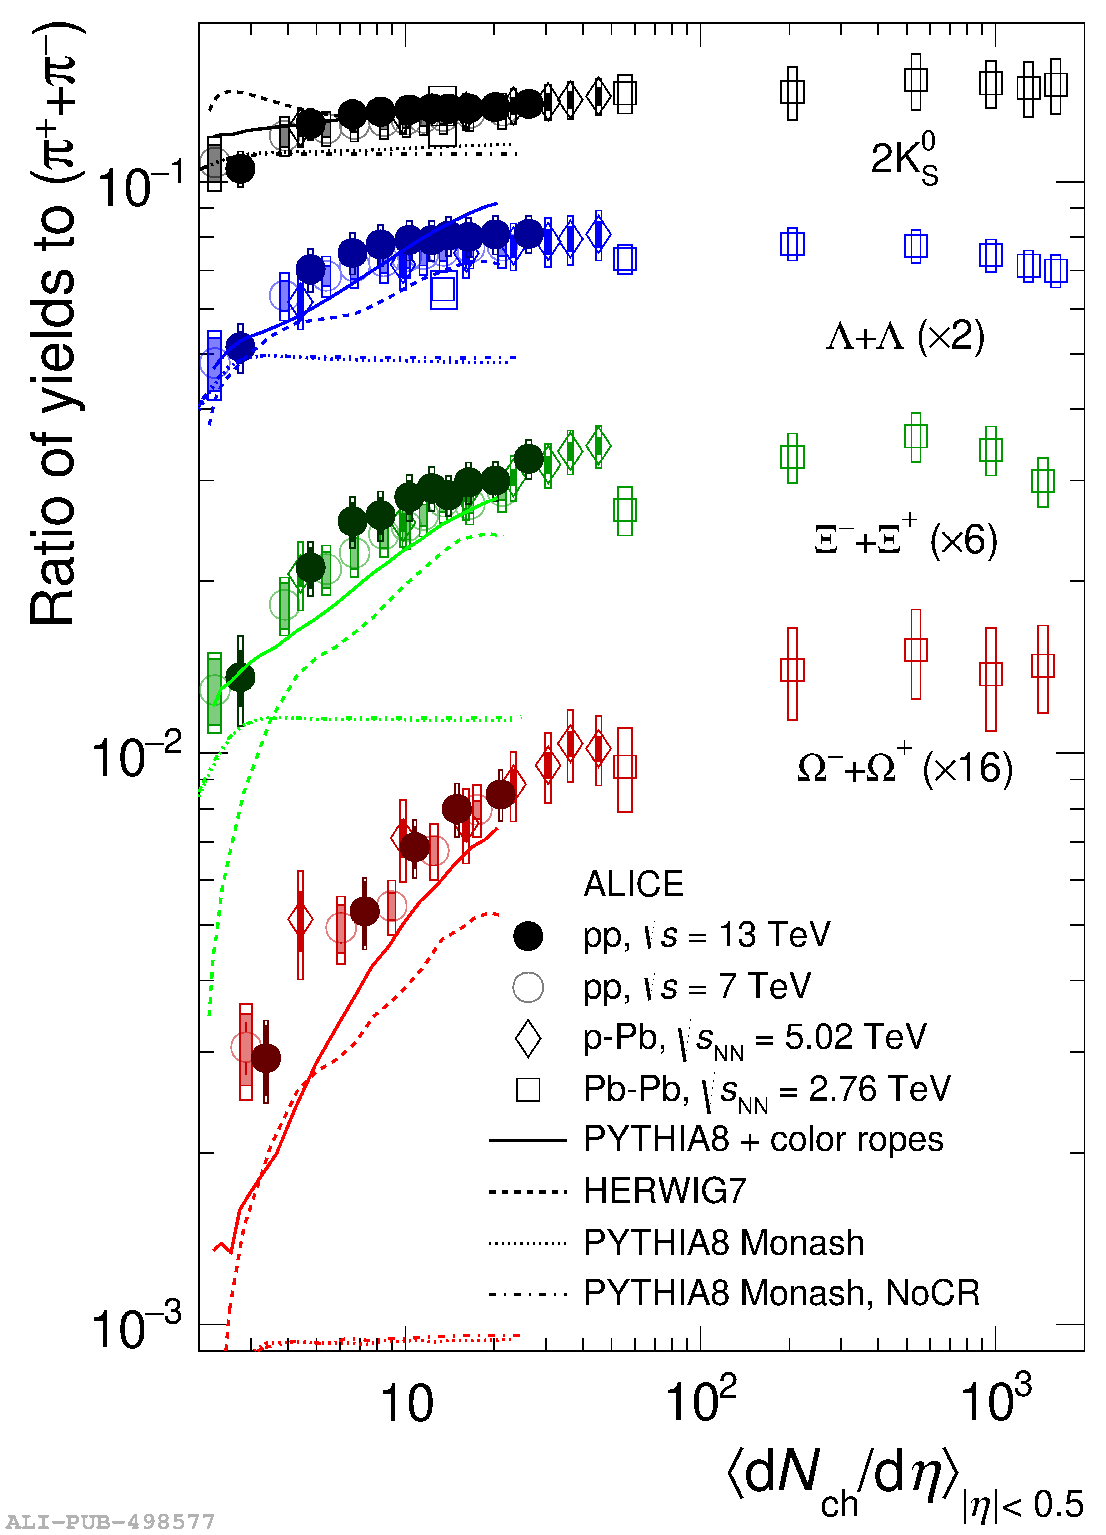
\includegraphics[width=0.5\linewidth]{images/HadronToPionRatio.pdf}
    \\
    \caption{Integrated strange hadron-to-pion ratios as a function of $\langle\textnormal{d}N_{\textnormal{ch}}/\textnormal{d}\eta\rangle$ in p-p, p-Pb
    and Pb-Pb collisions at ALICE\cite{Acharya:2020}.}
    \label{fig:had2pion}
\end{figure}

As is the case with p-Pb, a similar trend can be observed in p-p results with yield ratios steadily increasing as a function of multiplicity, seemingly
independent of collision system. The trend is best described by PYTHIA8 + color ropes approach, with other models varying in accuracy.

Baryon-to-meson ratios must also be evaluated for both strange and non-strange particles to rule out the possibility that the observed results are a mass
effect. $\Lambda/K_{\textnormal{\sc s}^{0}}$ and $p/\pi$ ratios are plotted in Fig. \ref{fig:bar2meson} to determine if there is any multiplicity dependence.
From the figure, it can be seen that the ratio curves are almost flat and no multiplicity dependence is observed, confirming that the enhancement is not
related to differences in hadron mass.

\begin{figure}[H]
    \centering
    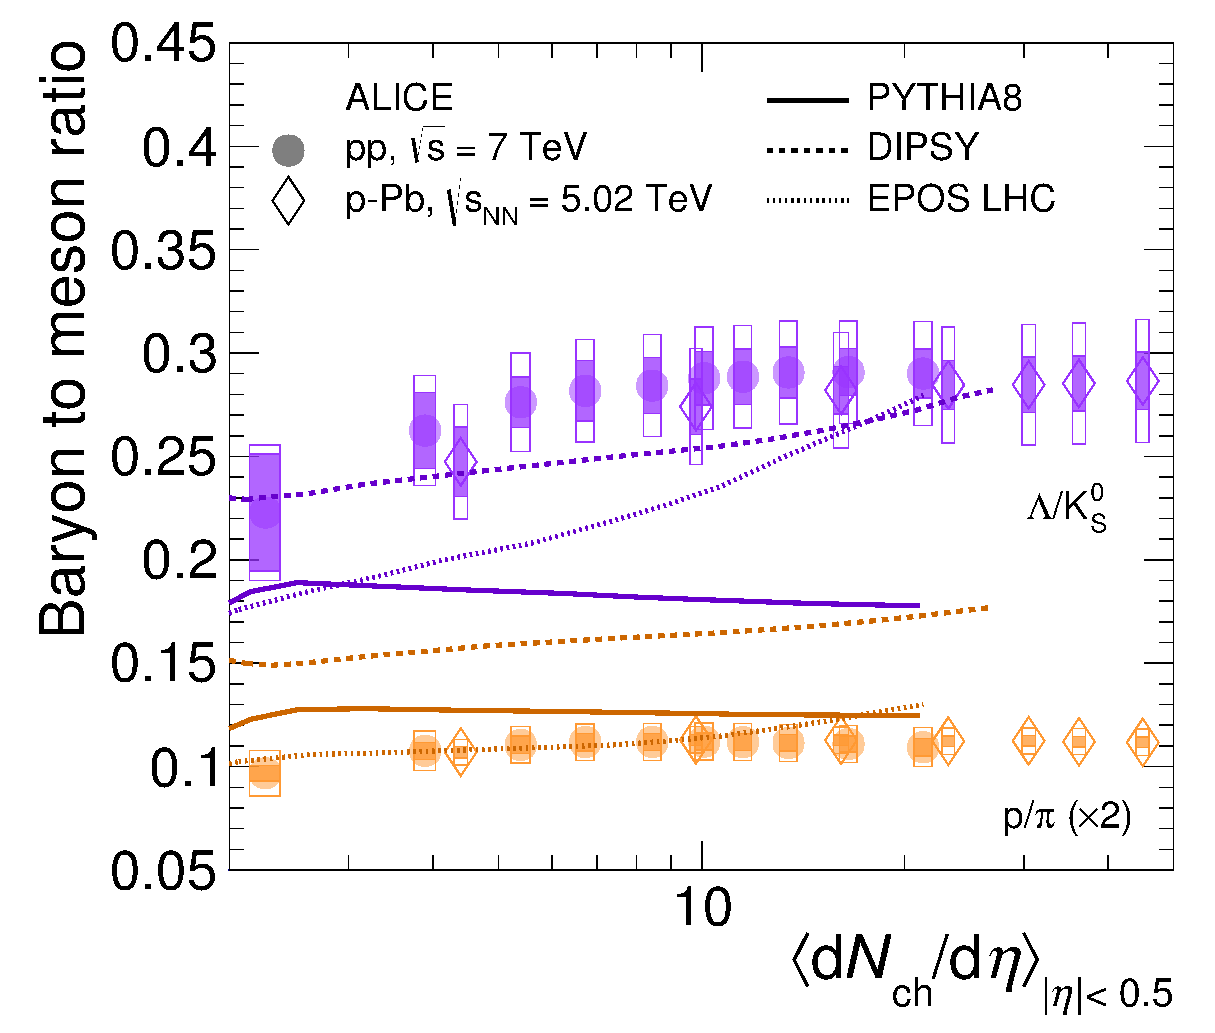
\includegraphics[width=0.7\linewidth]{images/bmratio.eps}
    \\
    \caption{Particle yield ratios $\Lambda/K^{0}_{\textnormal{\sc s}}$ and $p/\pi$ as a function of
    $\langle\textnormal{d}N_{\textnormal{ch}}/\textnormal{d}\eta\rangle$, ALICE\cite{nature:2016}.}
    \label{fig:bar2meson}
\end{figure}